\chapter{Design}
\label{cap:design}

\intro{In questo capitolo viene descritta la struttura dell'applicazione seguendo un approccio \textit{top-down}, partendo quindi dal \textit{frontend} per poi passare al \textit{backend} descrivendo \acrog{api} e \textit{database}.}

\section{Premessa}

Nonostante lo \textit{stage} si basasse sul lavorare ad un'applicazione già esistente, è stato comunque necessario realizzare uno studio riguardo la struttura di tale app, cercando di individuarne architettura e \textit{pattern} utilizzati. L'oggetto di questo capitolo, pertanto, non sarà la descrizione di un'architettura realizzata durante lo \textit{stage}, bensì la descrizione dell'architettura già presente nell'applicazione, alla quale mi sono dovuto adattare per effettuare le modifiche e aggiunte necessarie al progetto.\\
Ho ritenuto quindi l'approccio \textit{top-down} il più ragionevole da adottare, in quanto rispecchia la metodologia di studio da me seguita.

\section{Panoramica}

L'applicazione ha un'architettura a microservizi, come illustrato nella \figref{fig:microservizi}. Il suo funzionamento si basa su tre \textit{database} (CommonDb, SysDb e il \textit{database} aziendale contenente i dati da utilizzare) e due tipologie di \acrog{api} (\textit{gateway} e \textit{data provider}).\\
Per utilizzare l'applicazione è necessario effettuare una \textit{login}. Questa utilizza le \acrog{api} \textit{gateway} che interrogano il CommonDb, in particolare la tabella \texttt{Utente}, che contiene \textit{username} e \textit{password} di tutti gli utenti dell'applicazione.\\
Dopo aver effettuato la \textit{login} è possibile utilizzare l'app, e ogni volta che dei dati vengono caricati dal o nel \textit{database} aziendale viene messa in atto la seguente procedura:
\begin{enumerate}
    \item l'applicazione fa una chiamata alle \acrog{api} \textit{gateway};
    \item queste ricavano dal CommonDb l'url delle \acrog{api} \textit{data provider} dell'azienda associata all'utente registrato;
    \item viene effettuata una chiamata alle \acrog{api} dell'azienda (\textit{data provider}), le quali interrogano il SysDb, per ricavare i parametri di connessione al \textit{database} aziendale.
\end{enumerate}
I dettagli dell'architettura di ogni parte dell'applicazione verranno illustrati nelle sezioni seguenti.

\begin{figure}[H]
    \centering 
    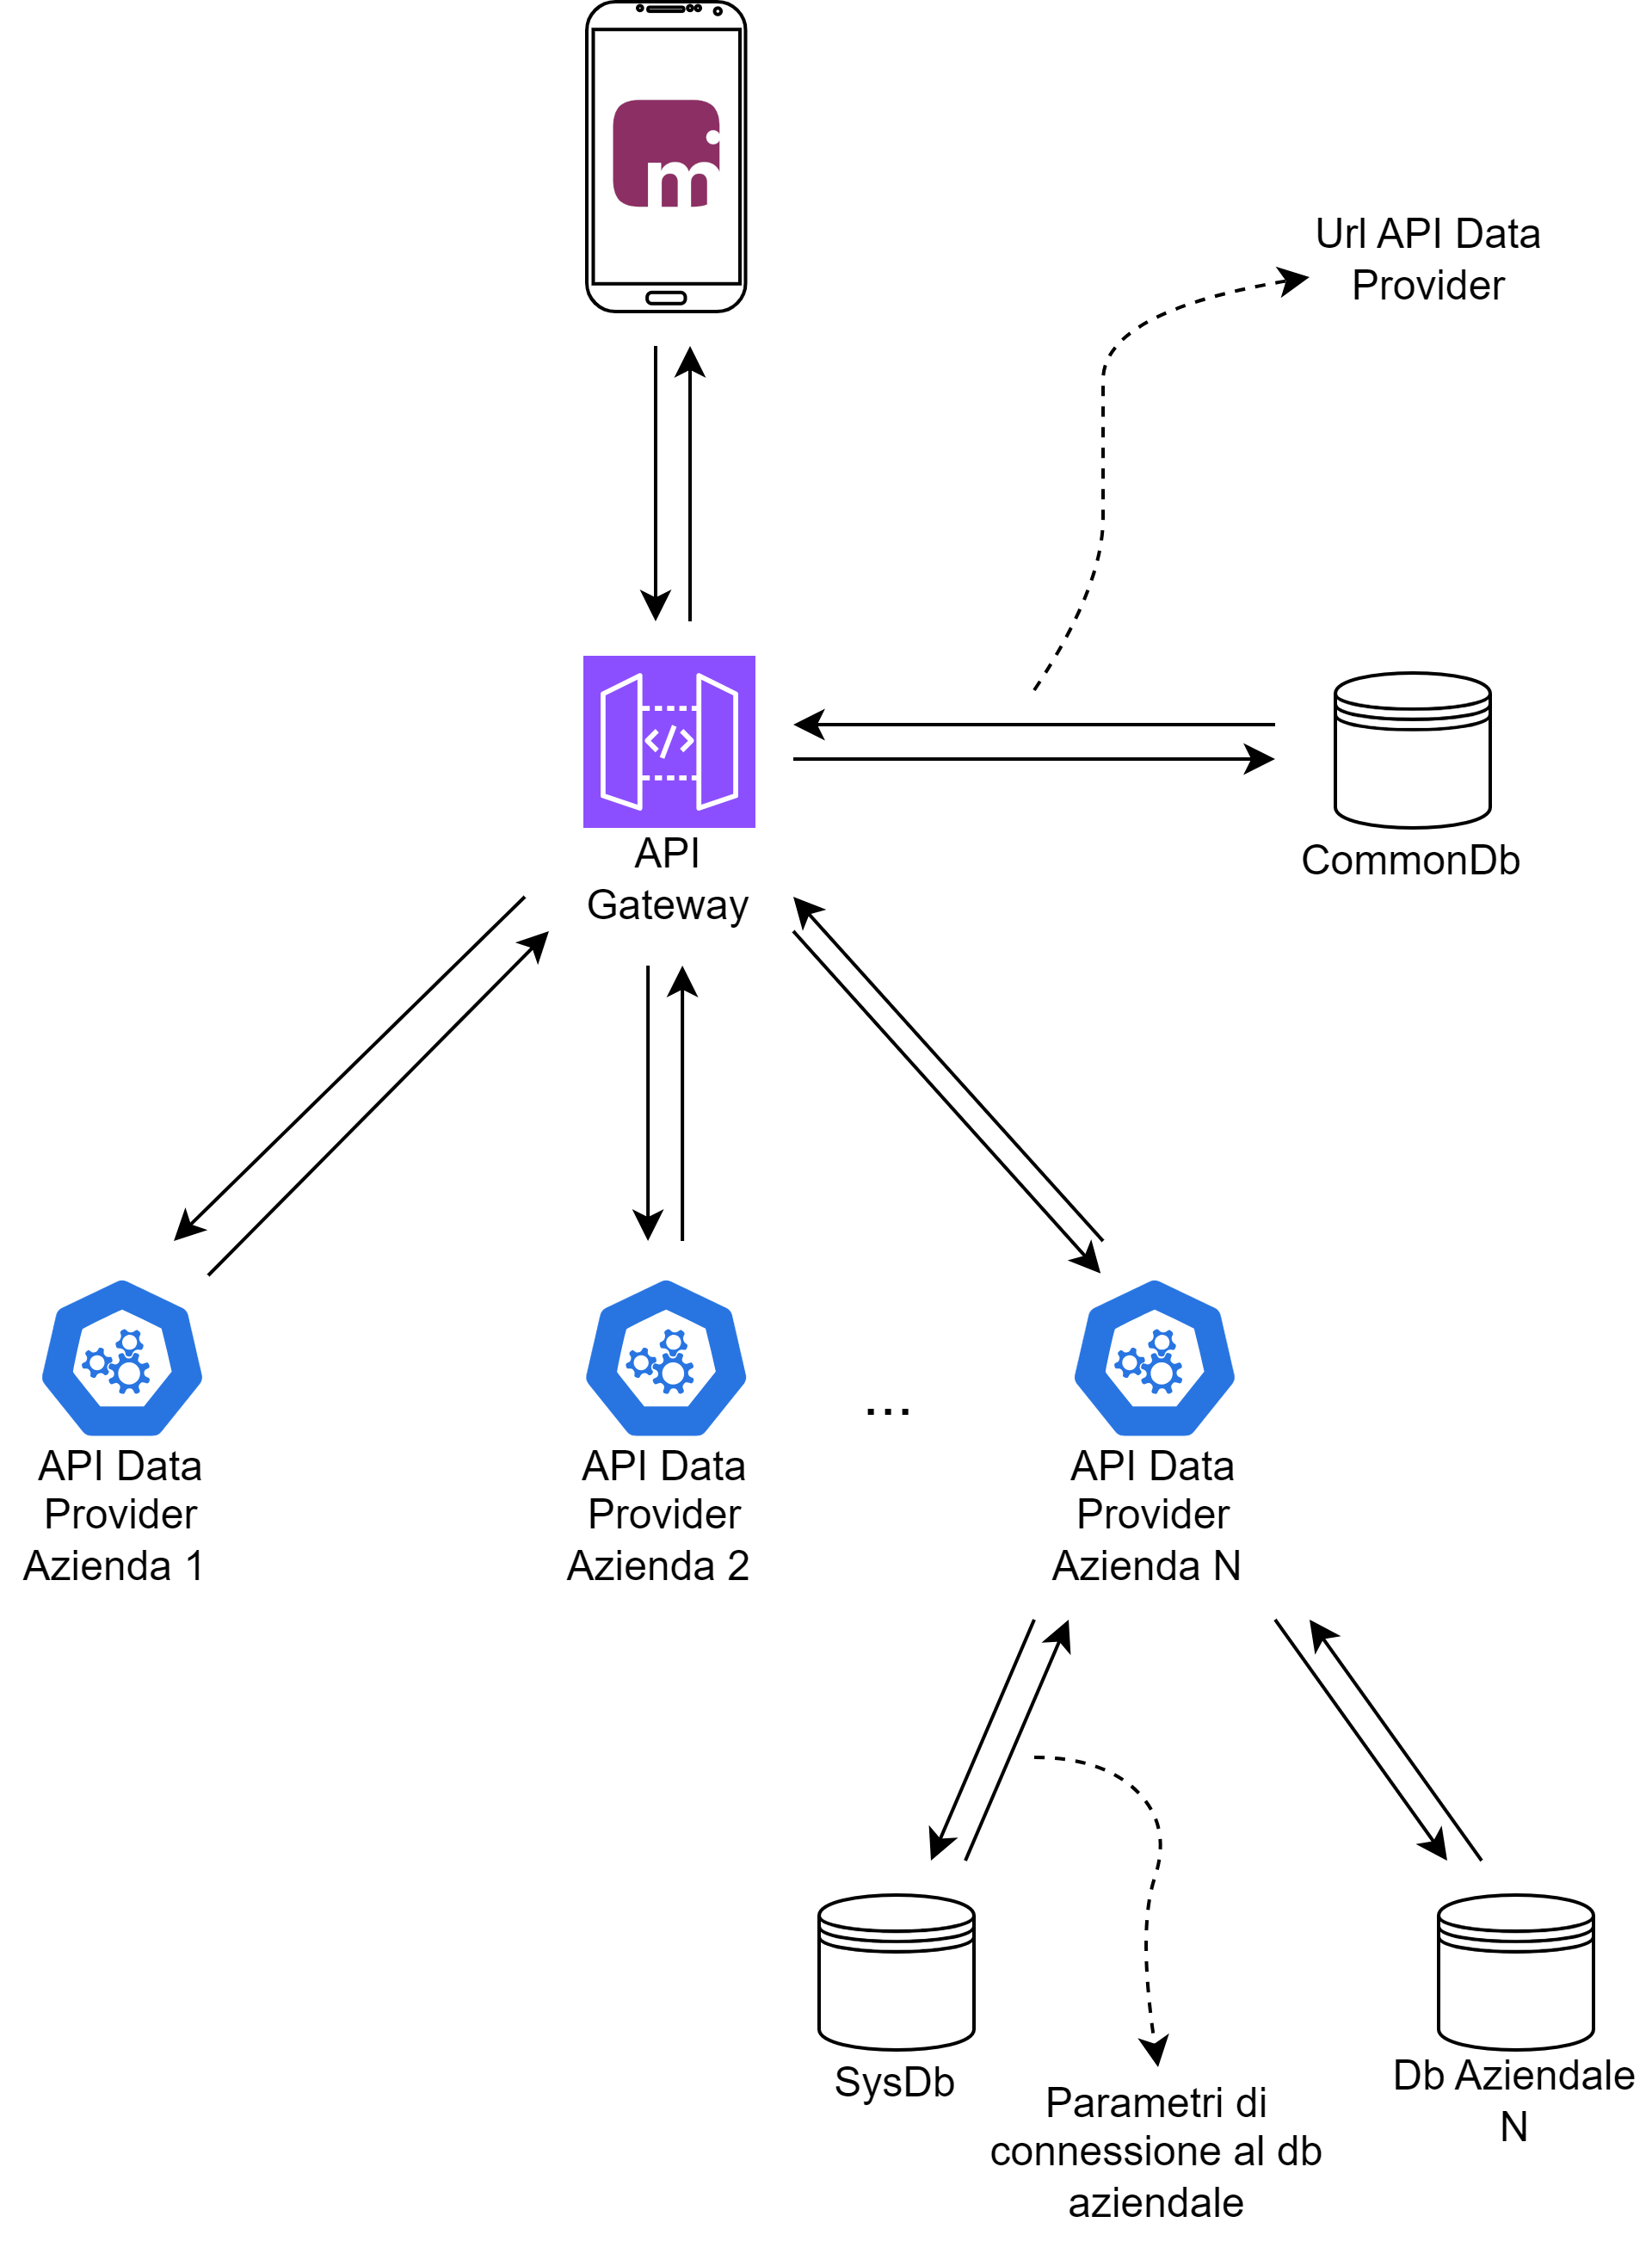
\includegraphics[width=.8\columnwidth]{images/architettura moviEXPENSE.png} 
    \caption{Architettura di moviEXPENSE}
    \label{fig:microservizi}
\end{figure}

\section{\textit{Frontend}}

Il \textit{frontend} di moviEXPENSE è stato realizzato con il framework Xamarin, il quale impone l'utilizzo del \textit{pattern} architetturale \textit{\textbf{Model-View-ViewModel}} (\textbf{MVVM}). Questo \textit{pattern} è molto utile per separare la logica dell'applicazione dall'interfaccia grafica, rendendo l'applicazione più semplice da modificare e testare. MVVM, infatti, separa il \textit{frontend} in tre parti:
\begin{itemize}
    \item \textbf{Model}: contiene tutte le classi dei dati di modello, ovvero tutti i dati strutturati che appartengono al dominio dell'applicazione;
    \item \textbf{View}: si occupa della rappresentazione grafica delle informazioni. Rappresenta dunque l'interfaccia utente, occupandosi della sua struttura e della sua presentazione;
    \item \textbf{ViewModel}: implementa le proprietà e i comandi con cui la View può effettuare dei \textit{data binding}. Presenta anche un sistema di notifiche verso la View che permette di segnalare ogni cambiamento che avviene ai dati durante l'esecuzione del programma.
\end{itemize}

\begin{figure}[H]
    \centering 
    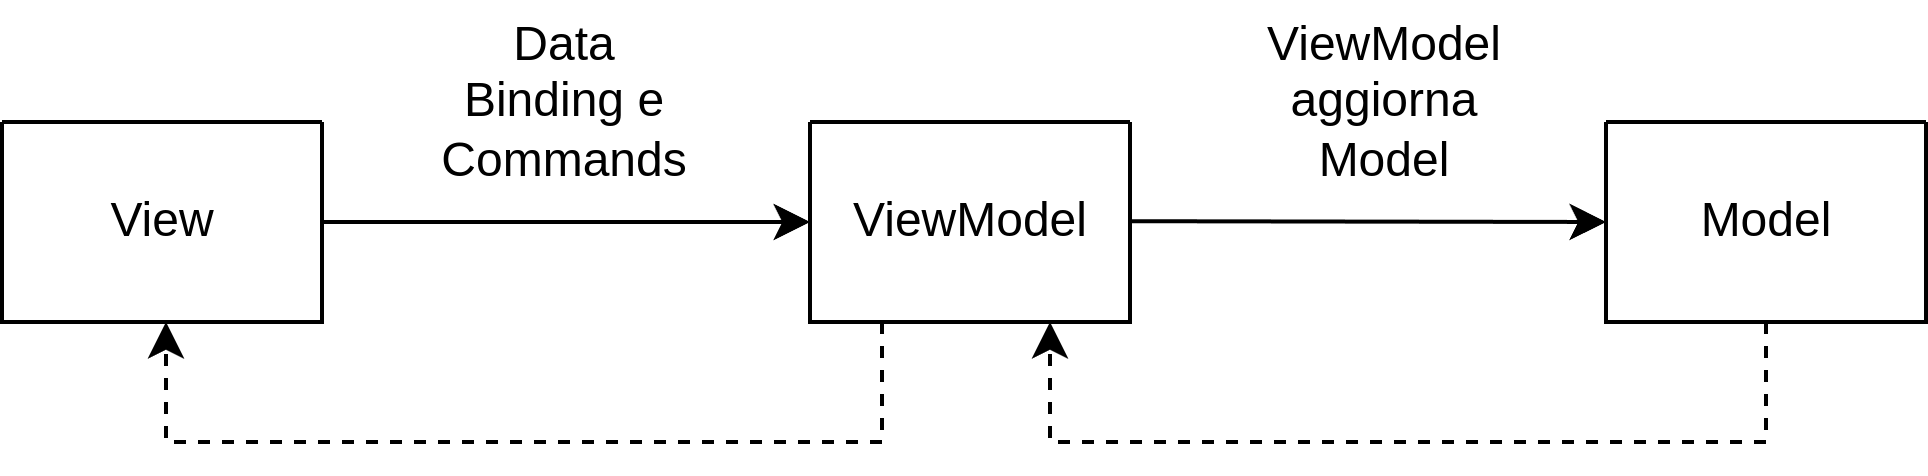
\includegraphics[width=.9\columnwidth]{images/MVVM.png} 
    \caption{Struttura del \textit{Model-View-ViewModel}}
\end{figure}

I tre \textit{namespace} principali del \textit{frontend} sono quindi:
\begin{enumerate}
    \item \texttt{MoviExpense.Models};
    \item \texttt{MoviExpense.Views};
    \item \texttt{MoviExpense.ViewModels}.
\end{enumerate}

\subsection{MoviExpense.Models}
\label{cap:model}

Questo \textit{namespace} contiene le classi che rappresentano gli oggetti di dominio dell'applicazione. Le quattro classi principali sono \texttt{User}, \texttt{Utente}, \texttt{Spesa} e \texttt{NotaSpese}.

\begin{namespacedesc}
    \classdesc{User}{è la classe utilizzata per l'autenticazione nel sistema. Contiene \textit{username} e \textit{password} presi dal form di \textit{login}, un booleano che conferma o meno il salvataggio delle credenziali e il \textit{\glox{token}} di autenticazione, inizialmente lasciato vuoto e assegnato quando l'identità viene confermata.}

    \classdesc{Utente}{rappresenta l'utente autenticato. È dotata di id, \textit{username}, codice utente, email, descrizione e il valore \texttt{TariKm}, che indica la tariffa di rimborso chilometrico per spese di carburante.}
    
    \classdesc{Spesa}{rappresenta l'oggetto principale dell'applicazione, ovvero la spesa che viene registrata. Contiene una serie di id oltre al proprio, che vanno ad identificare:
    \begin{itemize}
        \item la nota in cui è inserita;
        \item l'utente che registra la spesa;
        \item la causale;
        \item il tipo di pagamento;
        \item il fornitore presso cui è stata effettuata la spesa;
        \item la valuta con cui è stata effettuata.
    \end{itemize}
    \noindent Oltre a questi dati sono presenti le informazioni proprie della spesa, come l'importo, la data, il numero e la data della fattura, se emessa. Sono presenti poi alcuni \textit{flag} booleani che indicano se è presente una fattura, se la spesa è stata selezionata per essere inserita in una nota, se è rimborsabile e se è stata effettuata entro il comune di sede dell'azienda. Infine è presente un attributo che indica lo stato della spesa, il quale verrà spiegato nel dettaglio all'interno del prossimo capitolo.
    }

    \classdesc{NotaSpese}{modella una nota spese, ovvero un insieme di spese da inviare all'amministrazione dell'azienda. Ogni nota è identificata da un id, ed è dotata di:
    \begin{itemize}
        \item descrizione (ad esempio "Spese rimborsabili luglio 2024");
        \item data in cui viene effettuata;
        \item un \textit{check} che segnali se è una nota rimborsabile o meno;
        \item id dell'utente che registra la nota.
    \end{itemize}
    \noindent Sono presenti anche un \textit{flag} \texttt{IsEditable} che indica se la nota è modificabile e un intero che rappresenta lo stato della nota. Come per le spese, anche lo stato delle note sarà illustrato nel dettaglio nel prossimo capitolo.
    }
\end{namespacedesc}

\noindent All'interno del \textit{namespace} si trovano altre classi minori, che rappresentano attributi per le spese, come la causale, il tipo di pagamento o l'allegato, oppure altre entità dell'applicazione, ad esempio i totali delle spese divisi per determinate categorie.

\subsection{MoviExpense.Views}

Ogni classe di questo \textit{namespace} rappresenta una pagina dell'applicazione. Le pagine sono scritte utilizzando XAML, linguaggio prediletto di Xamarin.Forms, e per ogni file \texttt{.xaml} che definisce la struttura e l'aspetto della pagina, è presente un file \texttt{.xaml.cs} che inizializza tutte le componenti, carica le informazioni statiche nella pagina (ad esempio stringhe) e definisce i \textit{binding} con la ViewModel. Il nome di ogni file di questo \textit{namespace}, e di conseguenza ogni classe, termina con la parola "\texttt{Page}".

\begin{namespacedesc}
    \classdesc{LoginPage}{presenta il logo dell'applicazione e due \textit{entry} per inserire \textit{username} e \textit{password}.}
    \classdesc{HomePage}{contiene un breve testo di benvenuto e due pulsanti, uno per accedere alla pagina della spese, l'altro per accedere alla pagina delle note. In basso è presente una \textit{label} che mostra il numero di versione dell'app.}

    \classdesc{SpesePage}{mostra la lista della spese associate all'utente presenti nel \textit{database}. Queste sono filtrabili in base allo stato della spesa oppure possono essere mostrate tutte insieme. Da qui è possibile eliminare una spesa che sia ancora modificabile, visualizzarne i dettagli, creare una nuova spesa oppure accedere alla pagine di visualizzazione dei totali delle spese (\texttt{TotaliSpesePage}).}
    
    \classdesc{ViewEditSpesaPage}{questa pagina presenta una \textit{form} per la creazione, modifica o solamente visualizzazione di una spesa. Da questa pagina è possibile raggiungere le pagine di selezione (\texttt{SelCauPage}, \texttt{SelValutaPage}, \dots), nelle quali si possono selezionare alcuni campi della spesa, come la causale, la valuta, il tipo di pagamento e il fornitore.}
    
    \classdesc{NotePage}{offre le stesse funzionalità di \texttt{SpesePage} ma è basata sulle note spese associate all'utente e presenti nel \textit{database}. Non è possibile, però, visualizzare i totali.}
    
    \classdesc{ViewEditNotaPage}{permette di compilare una \textit{form} per la creazione di una nota spesa. Da qui si può accedere alla pagina \texttt{AddSpesePage}, utile ad inserire le spese desiderate nella nota, ed è possibile accedere alla visualizzazione dei totali di tali spese.}
\end{namespacedesc}

\subsection{MoviExpense.ViewModels}

Per ogni classe della View e del Model è presente una classe di ViewModel, in particolare queste sono distinte dal nome: le classi associate alla View hanno lo stesso nome che hanno nella View ma sostituiscono la parola "\texttt{Page}" finale con "\texttt{Manager}" (ad esempio a \texttt{ViewEditSpesaPage} corrisponde \texttt{ViewEditSpesaManager}), mentre quelle associate al Model hanno lo stesso nome che hanno nel Model ma preceduto da "\texttt{Vm}" (alla classe \texttt{Spesa} corrisponde la classe \texttt{VmSpesa}).\\
Le classi "\texttt{Vm}" sono utilizzate dalla ViewModel per comunicare con il Model. Hanno come attributo un oggetto del Model di cui effettuano il \textit{property wrap}, ovvero ne gestiscono i meccanismi di modifica e accesso. Questo permette di avere una migliore sincronizzazione dei dati tra Model e View, anche grazie al meccanismo di notifica presente in queste classi. Tutte le classi della ViewModel implementano l'interfaccia \texttt{INotifyPropertyChanged}, a cui appartiene il metodo \texttt{OnPropertyChanged} che permette di notificare alla View i cambiamenti nei dati del Model, così che possano essere effettuate le modifiche necessarie all'interfaccia grafica. Di seguito è riportato un esempio di \textit{property wrapping}:
\begin{minted}[linenos, breaklines, frame=lines, framesep=5mm]{csharp}
    public int IdSpesa
    {
        get => Spesa.IdSpesa;
        set
        {
            Spesa.IdSpesa = value;
            OnPropertyChanged(nameof(IdSpesa));
        }
    }
\end{minted}

\noindent Le classi "\texttt{Manager}", invece, effettuano il \textit{binding} con la View e si occupano di:
\begin{itemize}
    \item comunicare con le \acrog{api};
    \item gestire i dati non statici, ovvero di tutti i dati presi da \textit{database}, e che possono quindi subire modifiche durante l'utilizzo dell'app;
    \item gestire i comandi inviati dalla View. Ad esempio quando si clicca l'icona per eliminare una spesa, viene chiamato un metodo di una classe "\texttt{Manager}" della ViewModel.
\end{itemize}

\vspace{1.5cm}

\noindent Oltre ai tre \textit{namespace} appena descritti, ne sono presenti altri di supporto. Tra questi i principali sono: \texttt{MoviExpense.Converters} che contiene dei convertitori utili ad esempio ad assegnare proprietà booleane legate a valori non booleani, e \texttt{MoviExpense.Resources} che contiene tutte le stringhe dell'applicazione. L'immagine seguente riporta come viene visualizzato il file \texttt{Resources.resx} su Visual Studio.

\begin{figure}[H]
    \centering
    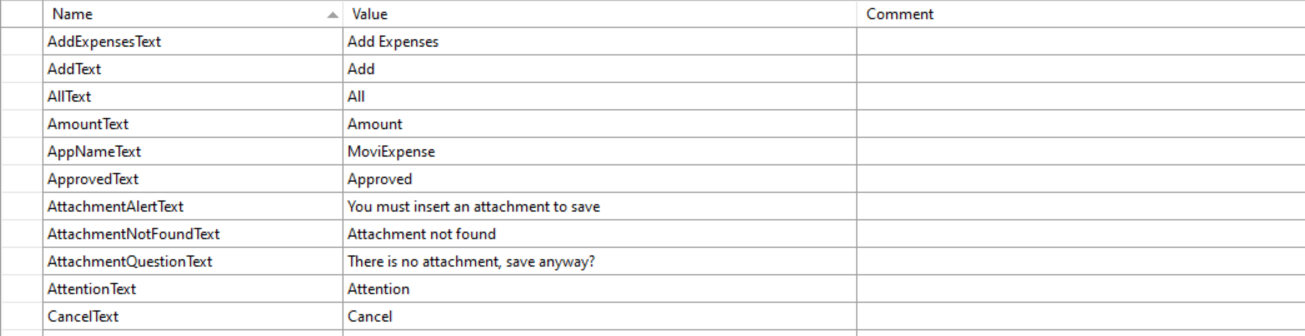
\includegraphics[width=\columnwidth]{images/resources.png}
    \caption{File Resources.resx aperto in Visual Studio}
\end{figure}



\section{\textit{Backend}}

\subsection{API}

Entrambe le \acrog{api} si basano su un'architettura \textit{layered} a tre livelli:
\begin{enumerate}
    \item \textit{\textbf{Presentation layer}}: livello di accesso a cui arrivano le chiamate;
    \item \textit{\textbf{Business layer}}: si occupa di elaborare le chiamate ed indirizzarle al \textit{database};
    \item \textit{\textbf{Data Access layer}}: livello che modella i dati del \textit{database} in oggetti di dominio.
\end{enumerate}

\noindent Il funzionamento generale delle \acrog{api} è il seguente:
\begin{enumerate}
    \item viene effettuata una chiamata http dall'esterno (dal \textit{frontend} o da un'altra \acrog{api});
    \item la chiamata viene intercettata da un oggetto \texttt{Controller} specifico che utilizza un oggetto \texttt{Service} per chiamare il metodo corrispondente alla chiamata http ricevuta;
    \item il \texttt{Service} "inoltra" la chiamata a una classe specifica del \textit{business layer};
    \item nel \textit{business layer} si utilizza un oggetto \texttt{ExpContext} per accedere al \textit{database};
    \item i dati prelevati o inseriti nel \textit{database} sono modellati con un oggetto del \textit{data access layer}.
\end{enumerate}

\noindent Di seguito è riportato il funzionamento delle \acrog{api} in modo \textit{top-down} attraverso i \textit{namespace} in cui avvengono le chiamate. Dato che entrambe le \acrog{api} funzionano in modo analogo, nei nomi dei \textit{namespace} sarà presente \texttt{[NomeAPI]}, che potrà essere quindi "\texttt{Gateway}" o "\texttt{DataProvider}".

\subsubsection{MoviExpense.Api.[NomeApi].Controllers}

È presente una classe \texttt{Controller} per ogni classe del modello (\texttt{SpesaController}, \texttt{CausaleController}, \dots). Questo \textit{namespace} rappresenta il livello di accesso alle \acrog{api}, è incaricato di accogliere le chiamate http emesse dall'esterno.\\
Ogni classe \texttt{Controller} ha un attributo della classe ad esso associata nel \textit{namespace} seguente e un metodo per ogni chiamata che possono ricevere. Questi metodi sono identificati tramite attributi di \textit{routing}, ad esempio la \texttt{Get} generale nella classe \texttt{SpesaController} ha il seguente attributo di \textit{routing}

\begin{minted}[linenos, breaklines, frame=lines, framesep=5mm]{csharp}
    [HttpGet] //Attributo di routing
    public IActionResult Get(int filterType, bool rimborsabile) {...}
\end{minted}

\noindent Anche la classe stessa è identificata da diversi attributi, in particolare:
\begin{itemize}
    \item \texttt{[Authorize]}: indica che è necessario essere autenticati per accedere alle funzionalità dell'\acrog{api};
    \item \texttt{[Route("api/[controller]")]}: specifica parte dell'url dell'\acrog{api};
    \item \texttt{[ApiController]}: consente di abilitare gli attributi di \textit{routing}, le risposte automatiche per i codici di errore 400 e il \textit{binding} con attributi come \texttt{[FromBody]}, \texttt{[FromForm]}, \dots
\end{itemize}

\noindent All'interno di ogni metodo costruiscono un oggetto di tipo \texttt{Param}, costituito da \textit{username} dell'utente e codice dell'azienda associata, e chiamano il metodo del \texttt{Service} corrispondente alla chiamata ricevuta. Nel caso della \texttt{Get} inserito prima viene
chiamato \texttt{\_service.GetAll(...)}, dove \texttt{\_service} è di tipo \texttt{ISpesaService}.

\subsubsection{MoviExpense.Api.[NomeApi].Services}
\label{cap:services}

È presente un'interfaccia e una classe concreta per ogni \texttt{Controller}, ad esempio sono presenti \texttt{ISpesaService}, \texttt{SpesaService}, \texttt{ICausaleService}, \texttt{CausaleService}, \dots\\
Ogni classe concreta ha come attributo un oggetto del \textit{business layer} tramite cui chiama il metodo corrispondente alla chiamata http ricevuta.\\
Continuando l'esempio iniziato precedentemente, ci sarà un oggetto \texttt{SpesaBL bl} che in un metodo \texttt{Get} chiamato dal \texttt{Controller} effettuerà la chiamata \texttt{bl.GetAll(...)}.

\subsubsection{MoviExpense.Api.[NomeApi].BL e MoviExpense.Api.[NomeApi].DAL}

\texttt{DAL} ha il compito di modellare i dati del \textit{database} in oggetti di dominio, di conseguenza avrà una classe per ogni tipo di oggetto (\texttt{Spesa}, \texttt{Causale}, \dots). Questi oggetti sono utilizzati nelle classi \texttt{BL}.\\
Nelle classi \texttt{BL} viene ricavata la stringa di connessione al \textit{database} aziendale tramite il \textit{database} Sys, e utilizzati degli oggetti \texttt{ExpContext} per effettuare la connessione ed eseguire le \textit{query} necessarie a soddisfare la chiamata http ricevuta.

\subsubsection{Gateway}

Il funzionamento delle \acrog{api} \textit{gateway} corrisponde a quello delle \textit{data provider} solamente per effettuare \texttt{Get} sui dati dell'utente autenticato e per effettuare l'autenticazione (in questo caso c'è solamente una chiamata ulteriore). In tutti gli altri casi, il loro funzionamento è uguale solamente fino alla sezione riguardante le classi \texttt{Service}. Quando la chiamata arriva a una classe del \textit{namespace} \texttt{MoviExpense.Api.Gateway.Services}, infatti, non viene inoltrata al \textit{business layer} ma viene ricavato dal CommonDb l'url delle \acrog{api} \textit{data provider} corrispondenti all'azienda dell'utente e la chiamata viene inoltrata a queste.

\paragraph{Autenticazione} Come detto in precedenza, le \acrog{api} \textit{gateway} in caso di autenticazione funzionano allo stesso modo delle \textit{data provider}, con una sola aggiunta. Quando si arriva al \textit{business layer}, dopo aver effettuato la \textit{query} sul CommonDb per verificare che l'utente esista e le credenziali siano corrette (utilizzando una classe del \textit{data access layer}), viene chiamato un metodo del \textit{namespace} \texttt{MoviExpense.Api.Gateway.Authentication}, che contiene la classe \texttt{Engine}. Questa classe permette la gestione dell'autenticazione tramite \acrog{jwt} ed è responsabile della generazione del \glox{token} di autenticazione per l'utente.


\subsection{\textit{Database}}

Come si può vedere nella \figref{fig:microservizi}, nel sistema dell'applicazione sono presenti tre \textit{database}: CommonDb, SysDb e un \textit{database} aziendale.

\subsubsection{CommonDb}

Viene utilizzato per:
\begin{itemize}
    \item autenticazione (tabella \texttt{Utente});
    \item recupero delle informazioni dell'utente (tabella \texttt{Utente});
    \item recuperare il numero di versione dell'applicazione (tabella \texttt{AppInfo});
    \item recupero dell'url delle \acrog{api} \textit{data provider} (tabelle \texttt{UtenteAzienda} e \texttt{Azienda}).
\end{itemize}

\subsubsection{SysDb}

Contiene una sola tabella chiamata \texttt{Azienda}, che viene utilizzata per ricavare i parametri utili a costruire la stringa di connessione per il \textit{database} aziendale.

\subsubsection{\textit{Database} aziendale}

La maggior parte delle tabelle presenti in questo \textit{database} sono autoesplicative e sono comunque già state spiegate in precedenza. L'unica informazione presente in più è la presenza delle tabelle \texttt{*GrpUtente}. Gli utenti dell'applicazione sono organizzati per gruppi. Ogni gruppo può avere accesso a determinate causali, tipi di pagamento e fornitori, di conseguenza sono presenti tutte le tabelle utili a collegare queste alla tabella \texttt{GrpUtente}, ad esempio \texttt{CausaleGrpUtente} definisce a quali causali hanno accesso i diversi gruppi utente.

\begin{figure}[H]
    \centering
    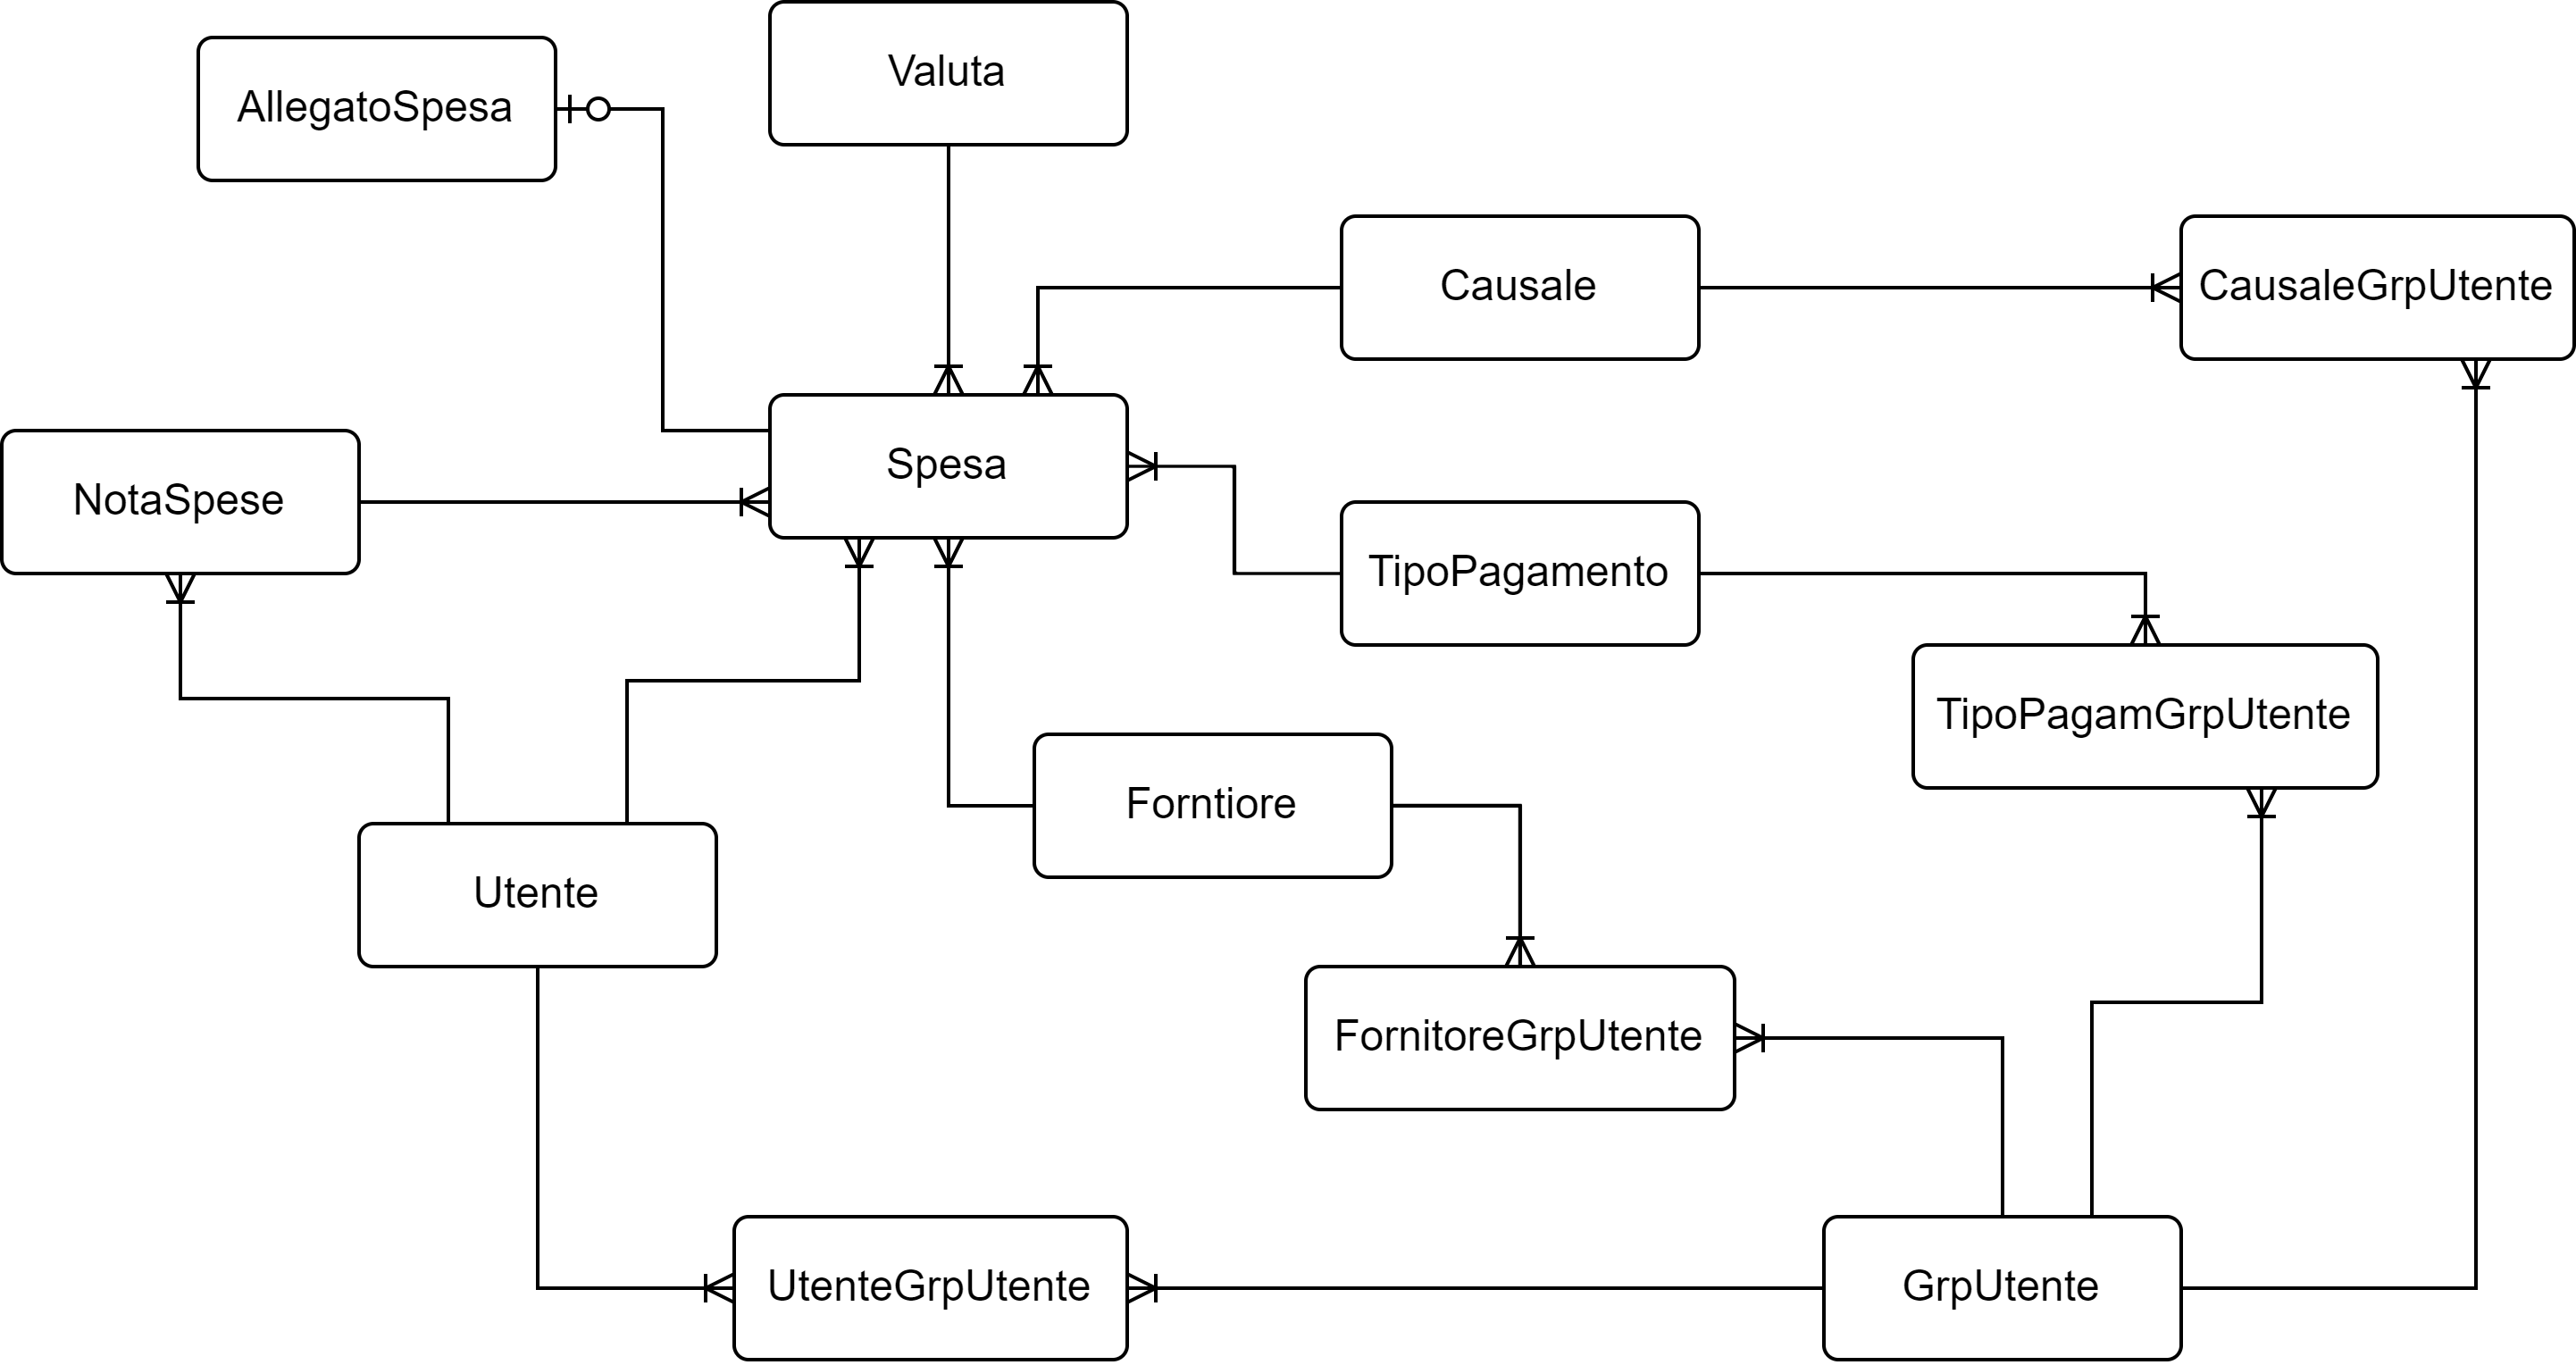
\includegraphics[width=\columnwidth]{images/ER moviEXPENSE.png}
    \caption{Schema entità-relazione \textit{database} aziendale}
\end{figure}
